\documentclass[12pt]{article}
\usepackage[top=1in, bottom=1in, left=1in, right=1in]{geometry}

\usepackage{setspace}
\onehalfspacing

\usepackage{amssymb}
%% The amsthm package provides extended theorem environments
\usepackage{amsthm}
\usepackage{epsfig}
\usepackage{times}
\renewcommand{\ttdefault}{cmtt}
\usepackage{amsmath}
\usepackage{graphicx} % for graphics files
\usepackage{tabu}

% Draw figures yourself
\usepackage{tikz} 

% writing elements
\usepackage{mhchem}

% The float package HAS to load before hyperref
\usepackage{float} % for psuedocode formatting
\usepackage{xspace}

% from Denovo Methods Manual
\usepackage{mathrsfs}
\usepackage[mathcal]{euscript}
\usepackage{color}
\usepackage{array}

\usepackage[pdftex]{hyperref}
\usepackage[parfill]{parskip}

% math syntax
\newcommand{\nth}{n\ensuremath{^{\text{th}}} }
\newcommand{\ve}[1]{\ensuremath{\mathbf{#1}}}
\newcommand{\Macro}{\ensuremath{\Sigma}}
\newcommand{\rvec}{\ensuremath{\vec{r}}}
\newcommand{\vecr}{\ensuremath{\vec{r}}}
\newcommand{\omvec}{\ensuremath{\hat{\Omega}}}
\newcommand{\vOmega}{\ensuremath{\hat{\Omega}}}
\newcommand{\sigs}{\ensuremath{\Sigma_s(\rvec,E'\rightarrow E,\omvec'\rightarrow\omvec)}}
\newcommand{\el}{\ensuremath{\ell}}
\newcommand{\sigso}{\ensuremath{\Sigma_{s,0}}}
\newcommand{\sigsi}{\ensuremath{\Sigma_{s,1}}}
%---------------------------------------------------------------------------
%---------------------------------------------------------------------------
\begin{document}
\begin{center}
{\bf NE 250, F15\\
October 21, 2015 
}
\end{center}

\textbf{Monte Carlo} for neutral particle transport

So far we've talked about the diffusion equation, derived the transport equation a few ways, and talked about the adjoint. \\
I'd like to spend the next bit of time talking about Monte Carlo methods, variance reduction, and how we can use the adjoint with variance reduction (note that I've totally just canned the syllabus). \\
After that we'll move into discretization and solution methods for the deterministic transport equation. 

What is Monte Carlo?
  \begin{itemize}
  \item The use of \textit{random processes} to determine a \textit{statistically-expected} solution to a problem
  \item Random processes can fulfill two roles:
  \begin{itemize}
    \item Statistical approximation to \textit{mathematical equations}
    \item Statistical approximations to \textit{physical processes}
  \end{itemize}   
  \item Construct a random process for a problem, 
  \item Carry out a numerical simulation by N-fold sampling from a (pseudo-)random \# sequence
\end{itemize}

For MC in radiation transport, we simulate many independent particles in a system:
\begin{itemize}
\item Treat each physical process as a \textit{probabilistic process}
\item \textit{Randomly sample} each process using an independent stream of pseudo-random numbers
\item Follow each particle from birth until it no longer matters
\item Accumulate the contributions of each particle to find the statistically-expected mean behavior and variance
\end{itemize}

\begin{figure}[h!]
\begin{center}
  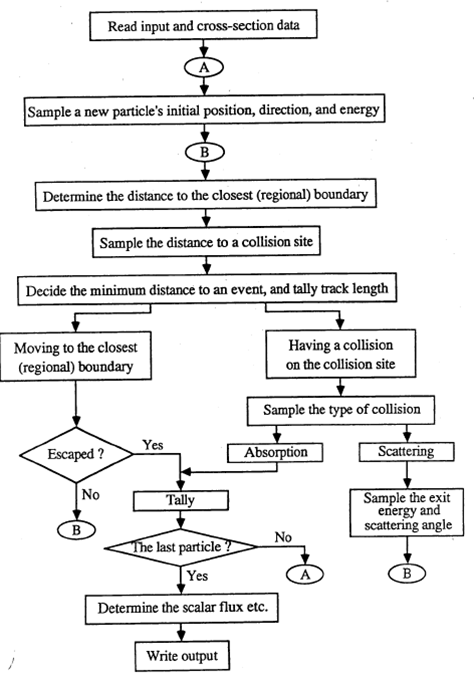
\includegraphics[height=6 in,clip]{../figs/MC-algorithm}
\end{center}
  \caption{Monte Carlo neutral particle transport algorithm}
  \label{fig:mc-algo}
\end{figure}

\textbf{WHY} use Monte Carlo?\\
Monte Carlo, when done properly, can be highly accurate and can be considered a ``gold standard" answer. Table~\ref{tab:comparison} compares MC and deterministic methods.
%
\begin{table}[h!]
\begin{center}
\begin{tabu}{| X | X |}
\hline
Monte Carlo         & Deterministic \\\hline
% -----------------------
* General geometry    & * Discretized geometry \\
* Continuous Energy   & * Multigroup in energy\\
* Continuous in Angle & * Angular Quadrature\\
* Number of particles governs solution accuracy & * Discretization and solver methods govern solution accuracy \\
* Must adequately sample phase space & * Must adequately discretize phase space \\
* Solutions have statistical error & * Solution contains truncation error\\
* \textbf{Local} solutions only; variable quality & * \textbf{Global} solutions; equal quality \\\hline
% -----------------------
* Easy to parallelize on CPUs & * Can be complicated to parallelize on CPUs\\
* Slow & * Can be quite fast \\
* Might be memory intensive & * Might be memory intensive \\
* Need efficient Variance Reduction & * Need acceleration methods \\\hline
  \end{tabu}
  \caption{Comparison of Monte Carlo and Deterministic Methods}
  \label{tab:comparison}
\end{center}
\end{table}
%
Figure~\ref{fig:mc-algo} shows the algorithm that is basically what happens in MC. \\
We will go through the very basics of the ideas about probability distributions, sampling, scoring, and statistics.

%-------------------------------------------------------
-------------------------------------------------------\\
\textbf{Probability Distributions}\\
We need to figure out all of these things about how particles are moving around in our system, but how do we do it?\\
We get functional expressions of the probability that various things will happen and try to take enough samples to effectively capture those expressions.
%
\begin{itemize}
\item For a random variable, $x$, the probability that $x$ will have a value between $a$ and $b$ is $P\{a \leq x \leq b\}$.
%
\item The \textit{probability density fuction} expresses the likelihood that $x'$ will take on a value between $x$ and $x+\Delta x$:
\begin{align*}
\lim_{\Delta x \to 0} f(x)\Delta x &= P \{ x \leq x' \leq x + \Delta x \}\\
\int_a^b f(x) dx &= P\{a \leq x \leq b\}
\end{align*}
%
\item We often normalize this PDF to integrate to one, using one of
\begin{equation}
\int_{-\infty}^{\infty} f(x) dx = 1 \quad \text{or} \quad
\int_{x^-}^{x^+} f(x) dx = 1 \nonumber
\end{equation}
%
\item To get the probability that our random variable $x'$ is less than or equal to some value $x$, we use a \textit{cumulative distribution function}:
\begin{align*}
F(x) &= P\{x' \leq x\} \\
F(x) &= \int_{-\infty}^{x} f(x') dx' \\
\lim_{x \to \infty} F(x) &\equiv F(\infty) = 1 \\
\lim_{x \to -\infty} F(x) &\equiv F(-\infty) = 0 \\
P \{ a \leq x' \leq b \} &= F(b) - F(a)
\end{align*}
\end{itemize}

Various physical phenomena can be represented by probability distributions
\begin{itemize}
  \item Photon emission energy: Each possible energy has a different probability (intensity)
  \item Scattering cross-sections:
    \item Each possible scattering angle has a different probability as a function of the energy
  \item Transmission through a medium: Probability of reaching a particular position
depends on the cross-section
\end{itemize}
%
We in one way or another get these PDFs and/or CDFs and use random numbers to select values for use in simulation.

%-------------------------------------------------------
-------------------------------------------------------\\
\textbf{Sampling}\\
Random sampling uses \underline{uniformly distributed random variables} ($\xi$ distributed between 0 and 1) to choose a value for a variable according to its probability density function.\\
Functionally, you can think of this as doing
\[
F(x) = \xi \quad \rightarrow \quad x = F^{-1}(\xi)\:.
\]
The trick then executing $F^{-1}$, which we cannot always do directly.\\
This gives rise to the need for a variety of sampling techniques (none of which we will really go into).\\
%
\textit{Basic} sampling techniques:
      \begin{itemize}
      \item Direct discrete sampling
      \item Continuous discrete sampling
      \item Rejection sampling
      \end{itemize}
\textit{Advanced }sampling techniques:
      \begin{itemize}
      \item Histogram
      \item Piecewise linear
      \item Alias sampling
      \item Advanced continuous PDFs
      \end{itemize}
%
The classic example of sampling in MC is the distance between collisions (which is a case where we can do direct inversion).
\begin{itemize}
\item $\Sigma_t$ = total macroscopic cross section of material
\[\Sigma_T = \sum_{j=1}^J N_j \sigma_t^j\]
%
\item The PDF for distance to collision is probability of interaction per unit distance $\times$ probability of traveling distance $s$ without interacting
\[f(s) = \Sigma_t \exp\bigl(-\Sigma_t s \bigr)\]
%
\item We integrate and normalize to get the CDF
\[F(s) = 1 - \exp\bigl(-\Sigma_t s \bigr)\]
%
\item To actually sample this, we invert it and get a random number (also noting that $\ln(1-\xi)$ is distributed the same exact way as $\ln(\xi)$ but the latter requires fewer operations:
\[
s = \frac{-\ln(\xi)}{\Sigma_t}
\]
\end{itemize}
%
If we're in a multi-region problem, we figure out if we intersect a boundary and if so move the particle to that boundary and determine how much farther it goes into the next material before having a collision.

After finding the location of the collision and the isotope collided with, we need to determine \textbf{what type of collision} occurs. 
%
\begin{itemize}
\item $\Sigma_t = \Sigma_{elastic} + \Sigma_{inelastic} + \Sigma_{capture} + \Sigma_{fission} + \dots$.
%
\item The probability of reaction of type $i$ for a given isotope is 
\[p_i = \frac{\Sigma_i}{\Sigma_t}\]
%
\item This gives a set of discrete probabilities, which we can sample 
\begin{itemize}
\item directly: generate $\xi$, determine $k$ s.t. $F_{k-1} \leq \xi \le F_k$, return $i = i_k$.
%
\item or by making an alias table and sampling.
\end{itemize}
\end{itemize}

%-------------------------------------------------------
-------------------------------------------------------\\
\textbf{Statistics}\\
The ``true" mean value, $\mu$, of and PDF is the expected value, $E(x)$
\[
\mu = E(x) = \int x f(x) dx
\]
Because we can't usually do this, we use random samples and estimate the true mean from the ``sample" mean, $\bar{x}$
\[
\bar{x} = \frac{1}{N}\sum_{i=1}^N x_i \qquad \lim_{N \to \infty} \bar{x} \rightarrow \mu\:.
\]
The variance of a PDF is the measure of spread in that PDF
\begin{align*}
\sigma^2 &= E[(x - \mu)^2] = \int (x - \mu)^2 p(x) dx \\
&= \int x^2 p(x) dx - 2 \mu \int x p(x) dx + \mu^2 \int p(x) dx\\
&= E(x^2) - \mu^2
\end{align*}
%
However, we don't know the PDF so we use the samples to get the sample variances
\begin{align*}
S_x^2 &= \frac{1}{N-1}\sum_{i=1}^N (x_i - \bar{x})^2 \\
&= \frac{1}{N-1} \biggl[\sum_{i=1}^N x_i^2 - 2 \bar{x}\sum_{i=1}^N x_i + \bar{x}^2 \sum_{i=1}^N 1 \biggr] \\
&\approx \bar{x^2} - \bar{x}^2
\end{align*}

\begin{figure}[h!]
\begin{center}
  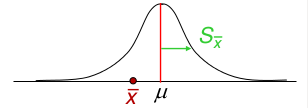
\includegraphics[height=1 in,clip]{../figs/gaussian}
\end{center}
  %\caption{Monte Carlo neutral particle transport algorithm}
  \label{fig:gaussian}
\end{figure}
%
The \underline{Central Limit Theorem} states that
For $N$ \textit{independent} random variables, $x_i$, sampled from \textit{identical distributions}, their mean follows a Normal (Gaussian) distribution.\\
(Note: this is the \textit{IID} requirement for MC)\\
We can use this information to define \textit{confidence intervals}
\begin{align*}
\bar{x} - S_{\bar{x}} &< E(x) < \bar{x} + S_{\bar{x}} \quad \text{about 68\% of the time}\\
\bar{x} - 2S_{\bar{x}} &< E(x) < \bar{x} + 2S_{\bar{x}} \quad \text{about 95\% of the time}
\end{align*}



%Use a random process to select a single value with the following requirements
%\begin{itemize}
%    \item Each sample should be independent from other samples
%    \item The PDF formed from a large number of samples should converge to the initial PDF
%    \item Recover the full resolution of the initial PDF
%\end{itemize}


%-------------------------------------------------------
-------------------------------------------------------\\
General purpose MC codes in nuclear:
\begin{itemize}
\item \textbf{MCNP}: developed at LANL, distributed via RSICC, \href{http://rsicc.ornl.gov}{http://rsicc.ornl.gov}
\item \textbf{Geant4}: developed by a large collaboration in the HEP community, \href{ http://geant4.web.cern.ch/geant4/}{http://geant4.web.cern.ch/geant4/}
\item \textbf{EGSnrc}: developed at NRC (Canada), \href{http://www.irs.inms.nrc.ca/EGSnrc/EGSnrc.html}{http://www.irs.inms.nrc.ca/EGSnrc/EGSnrc.html}
\item \textbf{SERPENT}: Developed by Dr. Jaakko Leppanen, VTT, Finland, \href{ http://montecarlo.vtt.fi/}{http://montecarlo.vtt.fi/}
\item \textbf{Shift}: developed at ORNL, distributed via RSICC, \href{http://rsicc.ornl.gov}{http://rsicc.ornl.gov}
\end{itemize}


%-------------------------------------------------------
%-------------------------------------------------------\\
%\textit{Analog}
%\begin{itemize}
%    \item Natural laws are \textbf{preserved}
%    \item The game is the ``analog" of the physical problem of interest (the history of each particle is simulated exactly)
%    \item No alteration of PDFs
%    \item At collision, particle is killed if absorption
%    \item Particle is born with weight 1
%    \item weight unchanged throughout history
%    \item Score when tallying events is 1
%\end{itemize}
%\textit{Non-Analog}
%\begin{itemize}
%    \item To reduce computation time, the strict analog simulation of particles is abandoned
%    \item Variance Reduction techniques: Absorption suppression, Russian Roulette (history termination), Splitting (history propagation), Forced collisions, Source biasing, Hybrid methods
%    \item Alter PDFs to favor events of interest
%    \item Particle can have different birth weight
%    \item Weight is altered if biased PDF is used
%    \item Particle survives ``absorption" and weight is changed
%    \item Splitting and RR can change weight
%    \item Score current weight when tallying
%\end{itemize}



\end{document}
